\section{Giới thiệu}

\begin{frame}{1. Giới thiệu}
CLIP là một bước đột phá trong AI đa phương thức (multi-modal AI), cho phép liên kết hình ảnh và ngôn ngữ.

\bigskip

CLIP (Contrastive Language–Image Pretraining) là mô hình thị giác–ngôn ngữ do OpenAI phát triển, nhằm học biểu diễn chung cho ảnh và văn bản. Nhờ phương pháp huấn luyện contrastive learning trên dữ liệu lớn, CLIP có khả năng thực hiện nhiều tác vụ mà không cần huấn luyện lại — gọi là zero-shot learning.
\end{frame}

\section{Nền tảng xây dựng mô hình CLIP}
\begin{frame}{2. Nền tảng xây dựng mô hình CLIP}
    \begin{itemize}
        \item Dữ liệu: WIT
        \item Kiến trúc mô hình: Dual-Encoder
    \end{itemize}
\end{frame}

\subsection{Bộ dữ liệu WIT}
\begin{frame}{2.1.1 Đặt vấn đề: Hạn chế của bộ dữ liệu truyền thống}
    \begin{block}{Bối cảnh}
        Các mô hình thị giác máy tính hàng đầu thường được huấn luyện trên các bộ dữ liệu được gán nhãn thủ công (ví dụ: ImageNet, MS-COCO).
    \end{block}

    \textbf{Hạn chế đáng kể:}
    \begin{itemize}
        \item Quy mô và chi phí hạn chế
        \item Phạm vi khái niệm cố định
        \item Thiếu ngữ cảnh và sắc thái
    \end{itemize}
\end{frame}

\begin{frame}{2.1.2 Động lực từ NLP và câu hỏi lớn}
    \textbf{Thành công của NLP:}
    \begin{itemize}
        \item Mô hình như GPT-3, BERT đã cách mạng hóa NLP nhờ huấn luyện trên khối lượng văn bản khổng lồ từ internet.
        \item Học từ dữ liệu "thô", không gán nhãn, bằng giám sát ngôn ngữ tự nhiên.
        \item Khả năng chuyển giao zero-shot vượt trội.
    \end{itemize}

    Liệu chúng ta có thể áp dụng triết lý tương tự để đạt được bước đột phá trong thị giác máy tính?
    
    $\Rightarrow$ Bộ dữ liệu WIT sinh ra để trả lời câu hỏi này.
\end{frame}

\begin{frame}{2.1.3 Bộ dữ liệu WIT (WebImageText)}
    WIT được xây dựng để trở thành nền tảng cho việc học biểu diễn hình ảnh từ ngôn ngữ tự nhiên.

    \bigskip
    \textbf{Quy mô}
    \begin{itemize}
        \item Bao gồm 400 triệu cặp (hình ảnh, văn bản) được thu thập từ internet.
        \item Lớn hơn 300 lần so với ImageNet và 4000 lần so với MS-COCO.
    \end{itemize}
    \bigskip
    \textbf{Lợi ích}
    \begin{itemize}
        \item \textit{Tiếp xúc đa dạng hơn:} Bao phủ một lượng lớn các khái niệm, đối tượng, hành động, phong cách nghệ thuật, và ngữ cảnh khác nhau.
        \item \textit{Giảm thiểu overfitting:} Lượng dữ liệu đồ sộ buộc mô hình phải học các khái niệm tổng quát hơn.
        \item \textit{Học hỏi sâu sắc hơn:} Khai thác tối đa tiềm năng của kiến trúc mạng sâu.
    \end{itemize}
\end{frame}

\begin{frame}{2.1.3 Bộ dữ liệu WIT (WebImageText)}
    \textbf{Bản chất giám sát:} Đây là điểm đặc biệt và cốt lõi nhất của WIT, sử dụng văn bản mô tả tự nhiên đi kèm với hình ảnh (\textbf{Natural Language Supervision}).
    
    \bigskip
    \textbf{Lợi ích}
    \begin{itemize}
        \item Tính đa dạng và khả năng khái quát hóa của khái niệm $\rightarrow$ Chìa khóa cho \textit{Zero-Shot Transfer}.
        \item Tiết kiệm chi phí
        \item Chấp nhận "nhiễu" tự nhiên vì dữ liệu từ internet không được gán nhãn thủ công một cách hoàn hảo.
    \end{itemize}
\end{frame}

\begin{frame}{2.1.3 Bộ dữ liệu WIT (WebImageText)}
\textbf{Chiến lược xây dựng}
\begin{itemize}
    \item Tìm kiếm cặp hình ảnh-văn bản dựa trên 500.000 truy vấn chọn lọc (từ Wikipedia, WordNet, v.v.) để đảm bảo tính bao quát.
    \item Đảm bảo rằng bộ dữ liệu bao phủ một \textbf{phạm vi rất rộng} các khái niệm, đối tượng, và tình huống khác nhau.
\end{itemize}
\end{frame}

\subsection{Kiến trúc mô hình}
\begin{frame}{2.2 Kiến trúc mô hình}
    CLIP bao gồm hai bộ mã hóa chính (dual-encoder) hoạt động độc lập để xử lý hai loại dữ liệu:
    \begin{itemize}
        \item \textbf{Image Encoder:} Chuyển đổi hình ảnh thành vector.
        \item \textbf{Text Encoder:} Chuyển đổi văn bản thành vector.
    \end{itemize}

    \textit{Mục tiêu:} Đưa cả hai vector này vào cùng một không gian nhúng đa phương thức.
\end{frame}

\begin{frame}{2.3 Image Encoder}
    CLIP thử nghiệm 2 dòng kiến trúc chính:
    \begin{itemize}
        \item ResNet (Residual Networks)
        \item Vision Transformer (ViT)
    \end{itemize}
\end{frame}

\begin{frame}{2.3.1 ResNet}
\begin{itemize}
    \item Kiến trúc CNN đột phá, nổi tiếng với kỹ thuật skip connections.
    \begin{figure}[H]
        \centering
        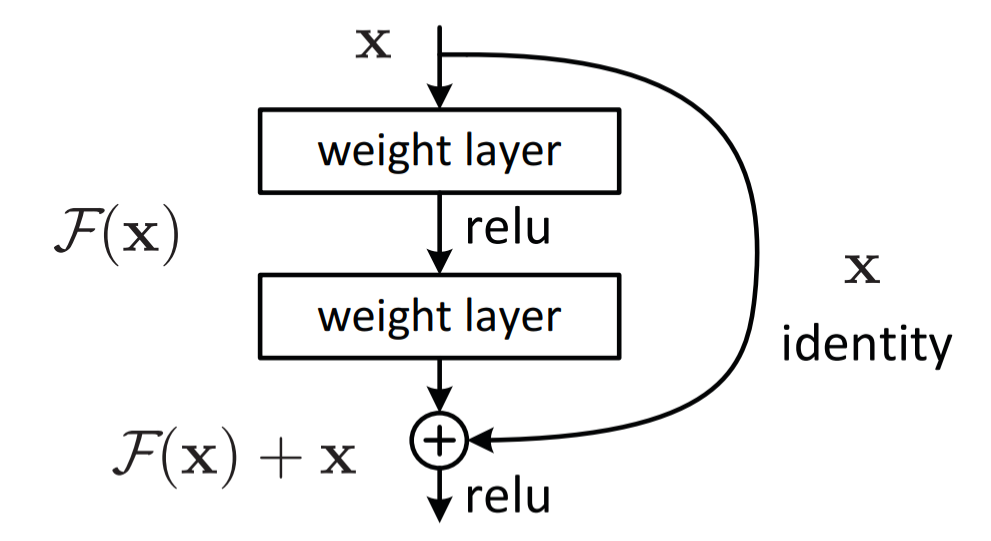
\includegraphics[width=0.5\textwidth]{img/01-skip_connection.png}
        \label{fig:skip_connection}
    \end{figure}
    \item CLIP sử dụng ResNet-50 và ResNet-101 làm cơ sở.
    \item Áp dụng một số cải tiến quan trọng.
\end{itemize}
\end{frame}

\begin{frame}{ResNet-50}
    \begin{figure}[H]
        \centering
        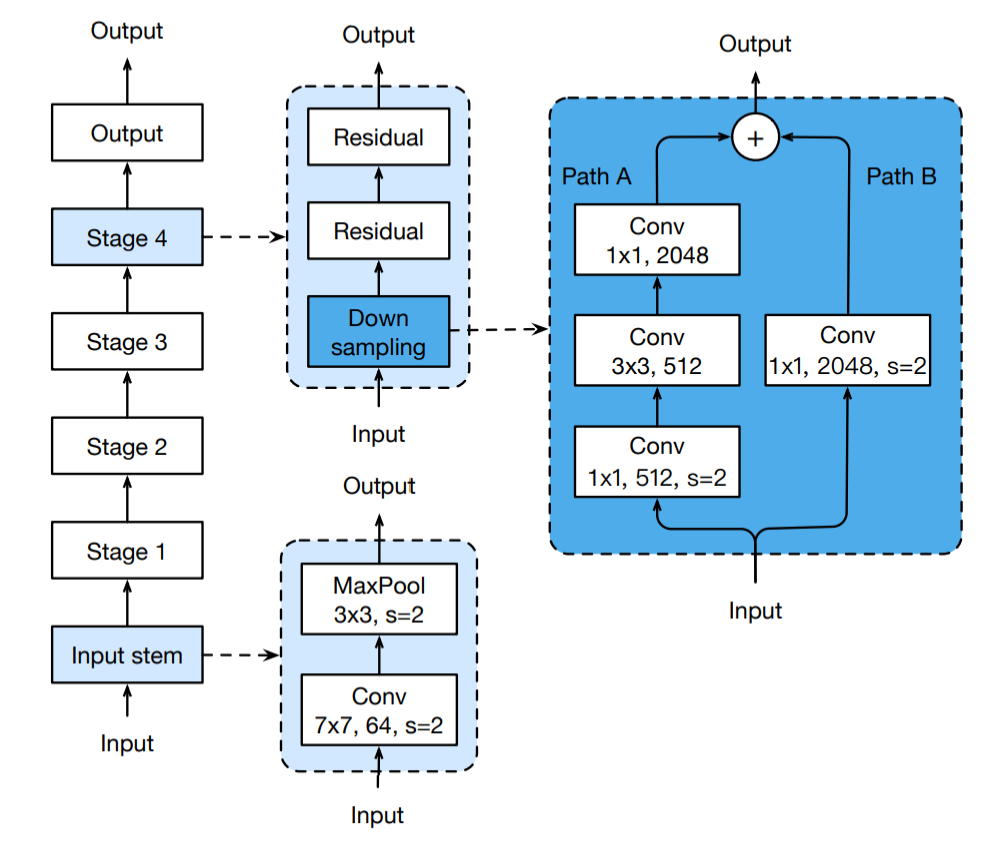
\includegraphics[width=0.5\textwidth]{img/01-resnet_50.png}
        \label{fig:resnet_50}
    \end{figure}
\end{frame}

\begin{frame}{ResNet-D}
\begin{figure}[H]
    \centering
    \begin{subfigure}[b]{0.25\textwidth}
        \centering
        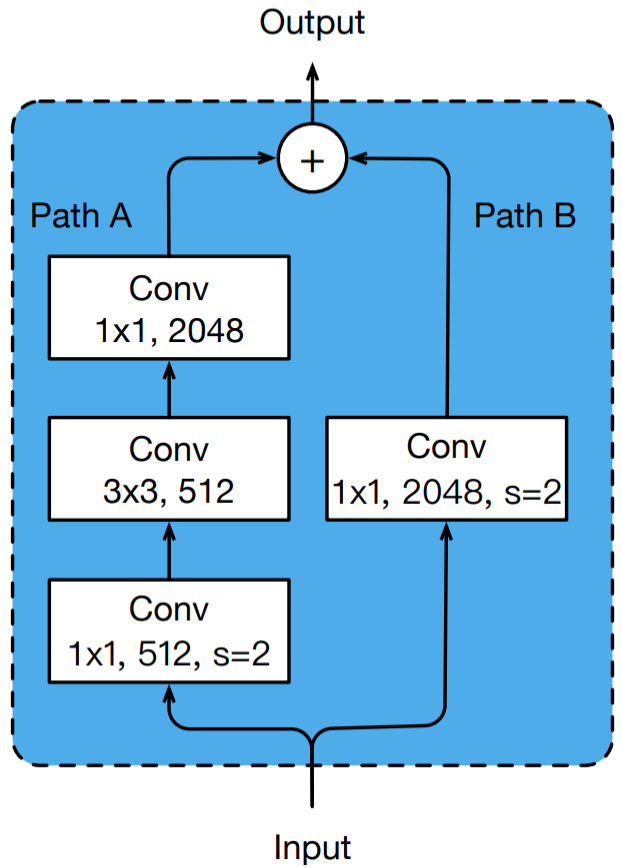
\includegraphics[width=\textwidth]{img/01-downsampling.png}
        \label{fig:skip1}
    \end{subfigure}
    \hspace{1cm}
    \begin{subfigure}[b]{0.25\textwidth}
        \centering
        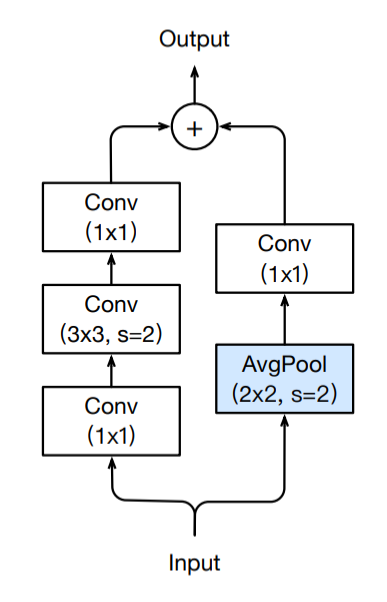
\includegraphics[width=\textwidth]{img/01-resnet_d.png}
        \label{fig:skip2}
    \end{subfigure}
    \label{fig:resnet_compare}
\end{figure}
\end{frame}

\begin{frame}{Anti-aliasing}
    \begin{figure}[H]
        \centering
        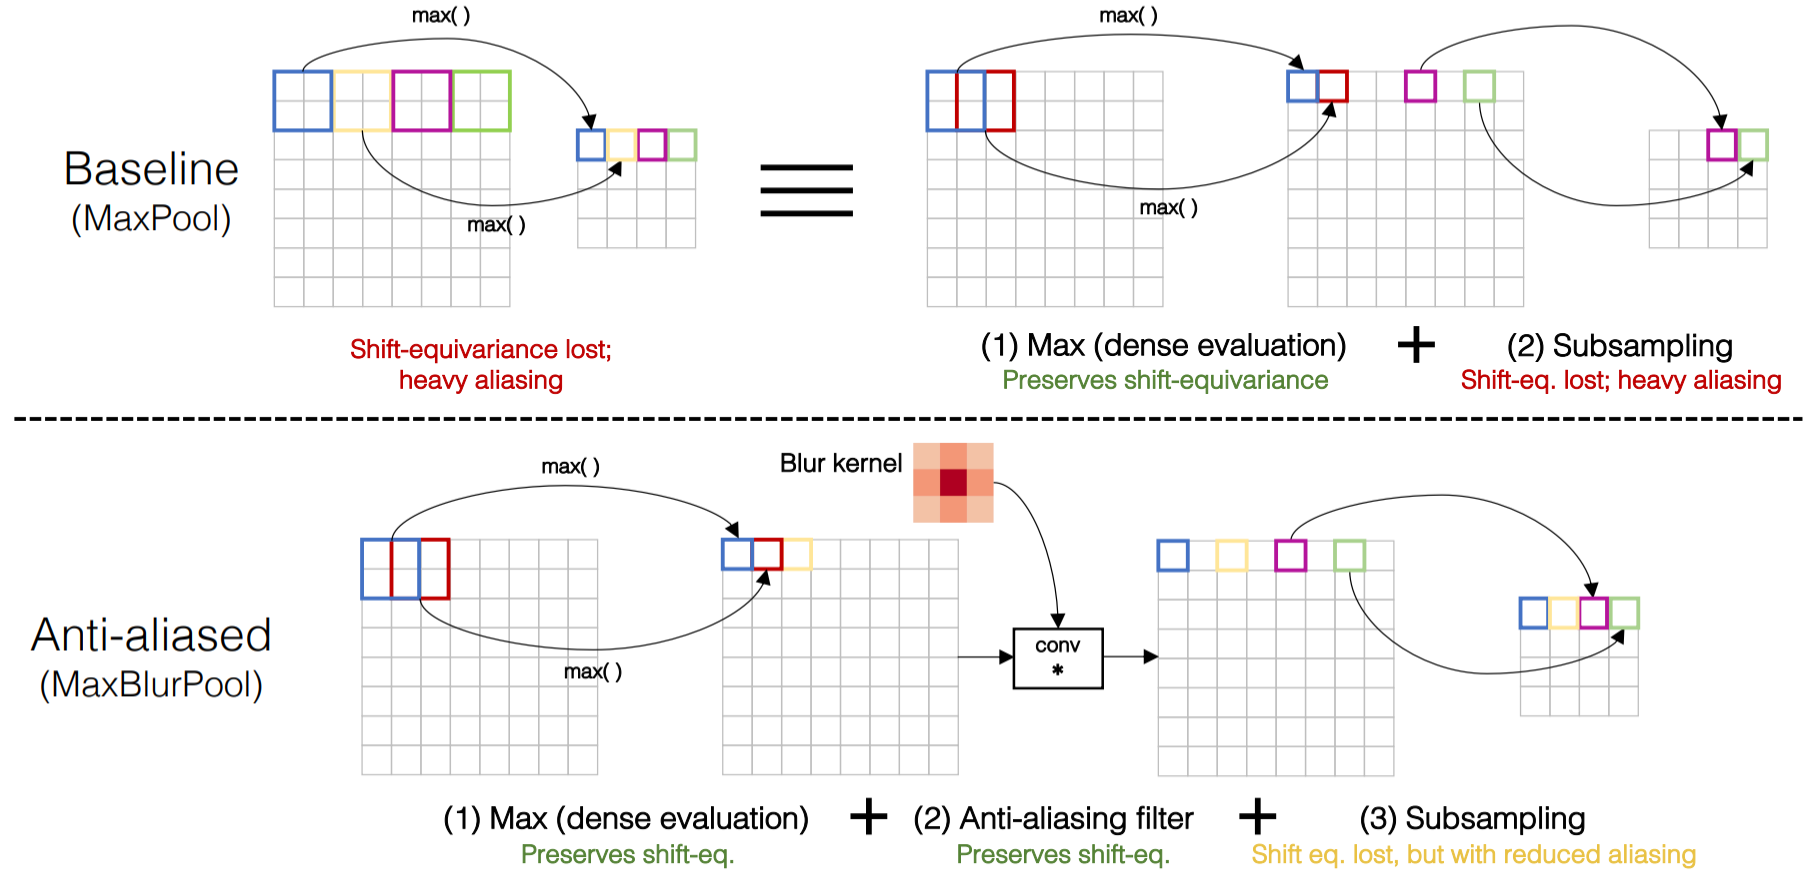
\includegraphics[width=0.8\textwidth]{img/01-anti_aliasing.png}
        \label{fig:skip_connection}
    \end{figure}

    \centering
    \begin{small}
        \textit{Making Convolutional Networks Shift-Invariant Again}, Richard Zhang
    \end{small} 
\end{frame}

\begin{frame}{Attention Pooling}
    Thay thế \textbf{Global Average Pooling} bằng \textbf{Attention Pooling}: Cho phép mô hình tập trung vào các vùng quan trọng nhất của hình ảnh khi tạo biểu diễn cuối cùng, thay vì chỉ lấy trung bình đơn giản.
\end{frame}

\begin{frame}{2.3.2 Vision Transformer}
    \begin{itemize}
        \item Kiến trúc mới hơn, dựa trên Transformer của NLP, hiệu quả vượt trội trên dữ liệu lớn.
        \item \textbf{Các sửa đổi nhỏ:} Thêm lớp Layer Normalization trước các khối Transformer, áp dụng lược đồ khởi tạo khác một chút.
        \item \textbf{Kỹ thuật huấn luyện:} Huấn luyện phiên bản ViT-L/14 lớn nhất thêm một epoch ở độ phân giải cao hơn (336x336 pixel) để tăng cường hiệu suất
    \end{itemize}
\end{frame}

\begin{frame}{Vision Transformer}
    \begin{figure}[H]
        \centering
        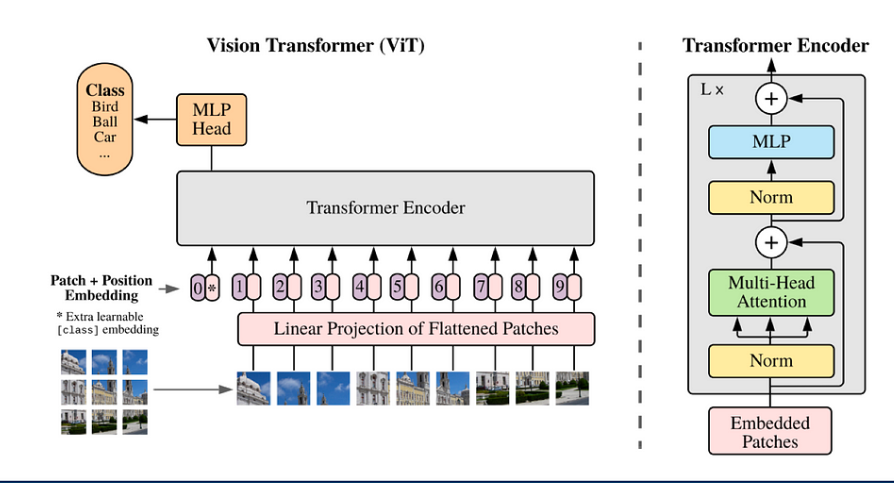
\includegraphics[width=0.8\textwidth]{img/01-transformer.png}
    \end{figure}
\end{frame}

\begin{frame}{2.4 Text Encoder}
    Sử dụng kiến trúc Transformer làm nền tảng cho bộ mã hóa văn bản, với một số điều chỉnh cụ thể.
\end{frame}

\begin{frame}{2.4.1 Kiến trúc nền tảng}
    \begin{itemize}
        \item Transformer chỉ có decoder, dựa trên Transformer gốc và cải tiến từ GPT-2.
        \item \textbf{Cấu hình điển hình:} 12 lớp, chiều rộng 512, 8 attention heads.
    \end{itemize}
\end{frame}

\begin{frame}{2.4.2 Text Tokenization}
\begin{columns}[c]
    \begin{column}{0.5\textwidth}
    \begin{itemize}
        \item Sử dụng thuật toán \textbf{Byte Pair Encoding} (BPE) để mã hóa từ.
        \item Sử dụng từ điển với 49152 từ vựng.
    \end{itemize}
    \end{column}

    \begin{column}{0.5\textwidth}
            \centering
            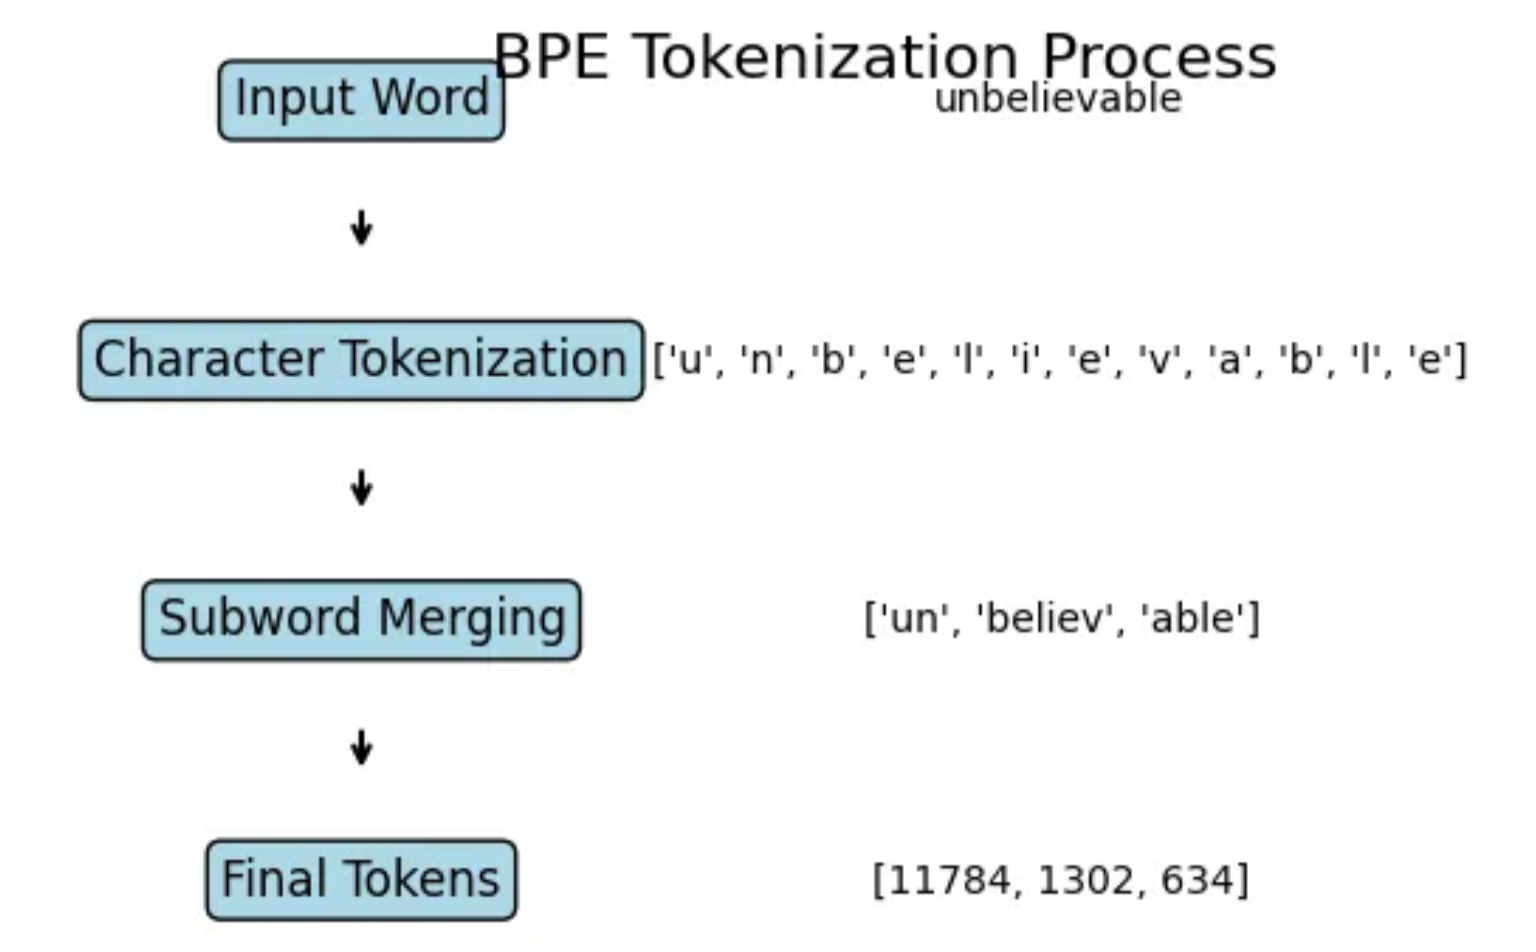
\includegraphics[width=\linewidth]{img/01-bpe.png}
    \end{column}
\end{columns}
\end{frame}

\begin{frame}{2.4.3 Masked Self-Attention}
Một cơ chế attention trong decoder Transformer đảm bảo rằng việc dự đoán
từ tiếp theo trong một chuỗi chỉ dựa trên các từ trước đó.

\bigskip
Tuy nhiên, CLIP không được huấn luyện để sinh văn bản, thay vào đó, CLIP học ghép cặp hình ảnh-văn bản lại với nhau. 

\bigskip
Cơ chế \textbf{Masked Self-Attention} được tận dụng để, ở mỗi lớp, mỗi token trong chuỗi đều có một vector biểu diễn ngữ cảnh riêng. Vector này không chỉ thể hiện bản thân token đó mà còn mã hóa thông tin về mối quan hệ của nó với các token trước đó trong chuỗi.
\end{frame}

\begin{frame}{2.5 Trích xuất đặc trưng}
    Trong số các vector biễu diễn ngữ cảnh sau khi qua lớp decoder, CLIP chọn \textbf{biểu diễn của token [EOS] ở lớp Transformer cuối cùng (lớp cao nhất)} do nó đã "nhìn thấy" tất cả các token trước nó và tổng hợp thông tin từ chúng.

    \bigskip
    Sau khi trích xuất, vector đặc trưng này được đưa qua LayerNorm và sau đó được chiếu tuyến tính vào một không gian chung. Đây là không gian mà các vector hình ảnh cũng được chiếu vào, cho phép tính toán độ tương đồng giữa văn bản và hình ảnh.    
\end{frame}

\begin{frame}{2.6 Mở rộng quy mô mô hình}
    CLIP cho thấy rằng hiệu suất tổng thể của nó không quá nhạy cảm với việc tăng số lượng tham số của bộ mã hóa văn bản.

    \bigskip
    Nhận thấy điều này, họ quyết định mở rộng quy mô tổng thể của mô hình để gia tăng hiệu suất. Chủ yếu tập trung vào việc mở rộng \textbf{chiều rộng} của bộ mã hóa văn bản một cách tương ứng với bộ mã hóa hình ảnh (ResNet hoặc ViT), nhưng \textbf{không tăng chiều sâu} (số lớp Transformer).
\end{frame}

\subsection{Tiền huấn luyện với Contrastive Learning}
\begin{frame}{3. Tiền huấn luyện với Contrastive Learning}
    Yếu tố then chốt tạo nên sự khác biệt về hiệu suất và khả năng mở rộng của CLIP so với các phương pháp trước đó trong việc học biểu diễn thị giác từ ngôn ngữ tự nhiên.
\end{frame}

\begin{frame}{3.1 Đặt vấn đề}
    Ban đầu, một số phương pháp học biểu diễn hình ảnh từ văn bản đã cố gắng xây dựng mô hình \textbf{dự đoán chính xác chú thích} của một hình ảnh.
    \bigskip
    
    Tuy nhiên, phương pháp này gặp phải một số thách thức lớn:
    \begin{itemize}
        \item Quá phức tạp và kém hiệu quả
        \item Tập trung sai mục tiêu
    \end{itemize}
\end{frame}

\begin{frame}{3.2 Giải pháp}
\begin{itemize}
    \item Proxy task - \textbf{Contrastive learning}
    \item Dự đoán cặp (hình ảnh, văn bản) nào là "đúng" trong một nhóm các lựa chọn.
\end{itemize}
\end{frame}

% \begin{frame}{3.3 Cơ chế hoạt động}
%     \begin{enumerate}
%         \item Tiền xử lý dữ liệu
%         \item Chuẩn bị Batch dữ liệu và mã hóa
%         \item Mã hóa song song
%         \item Tính toán ma trận tương đồng Cosine
%         \item Hàm mất má
%         \item Tối ưu hóa
%     \end{enumerate}
% \end{frame}

% \begin{frame}{3.4 Xây dựng batch đầu vào}
%     \begin{itemize}
%         \item Mỗi batch gồm $N$ cặp (hình ảnh, văn bản) thực tế được thu thập từ bộ dữ liệu WIT. Ví dụ: (Image$_1$, Text$_1$), (Image$_2$, Text$_2$), ..., (Image$_N$, Text$_N$).
%         \item Đây là $N$ cặp "đúng" (positive pairs).
%     \end{itemize}
% \end{frame}

% \begin{frame}{3.5 Tạo embedding vector}
%     \begin{itemize}
%         \item Image Encoder sẽ mã hóa ảnh đầu vào thành vector.
%         \item Text Encoder sẽ mã hóa văn bản đầu vào thành vector.
%     \end{itemize}
%     \bigskip
%     Các vector này sẽ được chiếu sao cho cùng kích thước và chuẩn hóa về độ dài bằng 1.
% \end{frame}

% \begin{frame}{3.6 Tính toán Similarity Matrix}
% \begin{columns}[c]
%     \begin{column}{0.5\textwidth}
        
%         Với $N$ embedding vector hình ảnh và $N$ embedding vector văn bản từ bước trên, chúng ta có thể tạo ra một ma trận độ tương đồng $S$ có kích thước $N \times N$. Các phần tử trên đường chéo chính là các cặp đúng.
%     \end{column}

%     \begin{column}{0.5\textwidth}
%         \centering
%         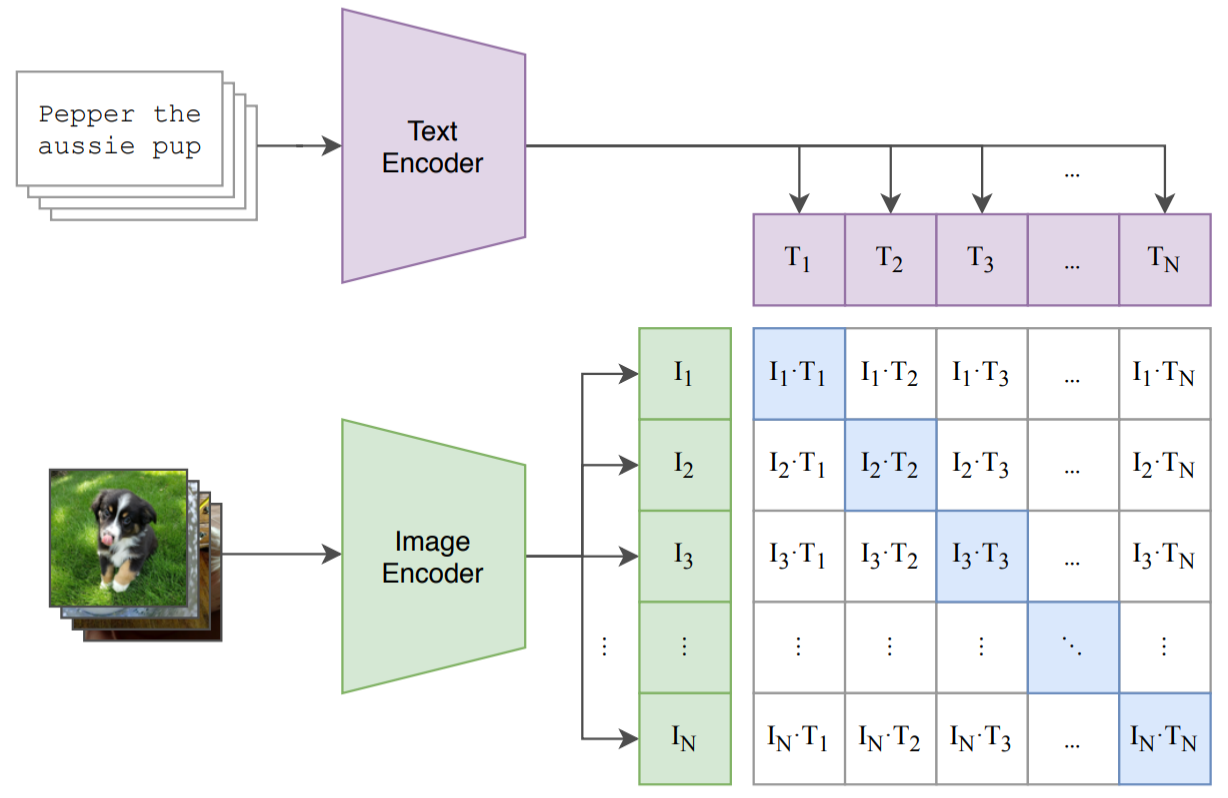
\includegraphics[width=\linewidth]{img/01-similarity_matrix.png}
%     \end{column}
% \end{columns}
% \bigskip
% Từng cặp hình ảnh-văn bản được tính bằng \textbf{cosine similarity} để đo độ tương đồng. Do các vector đã được chuẩn hóa, kết quả đơn giản là phép nhân vô hướng $I_i \cdot T_j^T$.
% \end{frame}

% \begin{frame}{3.7 Hàm mất mát và tối ưu hóa}
%     \begin{itemize}
%         \item Sử dụng một phiên bản của \textbf{N-pair Contrastive Loss} hoặc \textbf{InfoNCE Loss}, được gọi là \textbf{Symmetric Cross-Entropy Loss}.
%         \item \textit{Mục tiêu:} Tối đa hóa độ tương đồng của N cặp đúng và giảm thiểu độ tương đồng của $N^2$ – N cặp sai.
%         \item Tham số nhiệt độ (temperature parameter) được tối ưu hóa trực tiếp trong quá trình huấn luyện để kiểm soát độ "sắc nét" của sự phân biệt.
%     \end{itemize}
% \end{frame}

% \begin{frame}{3.8 Multi-modal Embedding Space - Sản phẩm cốt lõi}
%     \begin{itemize}
%         \item \textbf{Không gian thống nhất:} Một không gian vector cao chiều nơi biểu diễn của hình ảnh và văn bản có thể được so sánh trực tiếp.
%         \item \textbf{Phản ánh mối quan hệ ngữ nghĩa:}
%         \begin{itemize}
%             \item Các cặp có mối quan hệ sẽ có các vector nằm rất gần nhau (độ tương đồng cosine cao).
%             \item Các cặp không liên quan  sẽ có các vector nằm xa nhau (độ tương đồng cosine thấp).
%         \end{itemize}
%         \item \textbf{Khả năng "Open-set":} Vì được học từ dữ liệu ngôn ngữ tự nhiên đa dạng (WIT), không bị giới hạn bởi các lớp cố định. Có thể hiểu các khái niệm chưa từng thấy trong huấn luyện nếu có mô tả bằng ngôn ngữ tương ứng.
%     \end{itemize}
% \end{frame}